\documentclass[12pt]{article}

\usepackage[margin=1 in]{geometry}

%Use Times New Roman font
%\usepackage{pslatex}

% allow text colors
\usepackage[usenames,dvipsnames,svgnames,table,x11names]{xcolor}

%allow double-spacing
\usepackage{setspace}

%enable support for figures
\usepackage{graphicx}

\usepackage{rotating}
\usepackage{multirow}

\usepackage{url}

%handle filenames better
\usepackage{grffile}

%math
%\usepackage{mathtools}
\usepackage{amsmath}
\usepackage{amsfonts}
\usepackage{lipsum}

%control figure movement
\usepackage{placeins}

%center captions
\usepackage{caption}

%circuits and units
\usepackage[free-standing-units]{siunitx}
\DeclareSIUnit\vrms{\volt{}_{RMS}}
%\usepackage[americanvoltages,americancurrents]{circuitikz}
%\usetikzlibrary{calc}

% make scientific notation easy
\providecommand{\e}[1]{\ensuremath{\times 10^{#1}}}

% include pdf documents
\usepackage{pdfpages}

%for loops
\usepackage{pgffor}

%indent after new sections
\usepackage{indentfirst}

\usepackage{verbatim}

% allow greek letters outside math mode. \text<name of letter>
%\usepackage{textgreek}

% margin editing
\usepackage{changepage}

% braket notation, other goodies
\usepackage{physics}
\usepackage{braket}

%source code
\usepackage{listings}

%hyperlink support
\usepackage{hyperref}

% bibtex support
\usepackage{natbib}

%settings for Python code
%\lstset{basicstyle=\footnotesize\ttfamily,
%commentstyle=\color{OliveGreen},
%keywordstyle=\color{blue},
%tabsize=4,
%numbers=left,
%stringstyle=\color{red},
%language=Python,
%inputencoding=utf8,
%extendedchars=true,
%showstringspaces=flase,
% }

\begin{document}
\singlespacing
\title{Final Report\\
AST 383}
\date{Dec 15 2015}
\author{Robert Rosati \\ Mar\'{i}a Jos\'{e} Bustamante Rosell}
\maketitle

\begin{abstract}
\par Blah blah blah. Clusters are pretty man.
\end{abstract}

\doublespacing
\section{Motivation}

\section{Clustering Algorithms}
\par For our final project we decided to implement and compare the robustness of two density-based clustering algorithms under variations of user-defined parameters. 
Clustering algorithms have a wide variety of applications that range from satellite image segmentation, noise filtering and outlier detection, prediction of stock prices to bioinformatics. In particular, they are of high importance in astronomy when trying to identify dark matter halos and sub-halo structure.
There is a wide range of clustering algorithms out there for the taking. When handling large amounts of particles (in the order of trillions) the question of simplicity an easy parallelization arises also as a defining criterion. Both of the algorithms compared here are quite simple and easy to parallelize. \texttt{DBSCAN} is currently implemented on the latest halo-finders being developed \cite{BDCATS} and \textt{FIDEPE}, being quite a new algorithm, still has no implementation on cosmology (at least that we know of), the more reason to explore the code's performance.


\subsection{\texttt{DBSCAN}}

The \texttt{DBSCAN} (Density-Based Spatial Clustering of Applications with Noise) algorithm is a version of \texttt{FOF} (Friends of Friends) in which, unlike the former, the local density of a point is taken into consideration. This algorithm classifies points as being core points, density-reachable points and outliers. This classification is based on two user defined parameters: the radius of your neighborhood ($\epsilon $) and the minimum amount of points within it ($minPts$).

\begin{itemize}
\item A point $p$ is a core point if at least $minPts$ points are within distance $\epsilon$ of it (in it's neighborhood). Those points are said to be directly reachable from $p$. No points are reachable from a non-core point.
\item A point $q$ is reachable from $p$ if there is a path $p_1, ..., p_n$ with $p_1 = p$ and $p_n = q$, where each $p_{i+1}$ is directly reachable from $p_i $(so all the points on the path must be core points, with the possible exception of $q$).
\item All points not reachable from any other point are outliers.
\end{itemize}

Once a core point is selected, all the points reachable from it will be tagged as part of the same cluster.

\begin{figure}[ht]
\centering
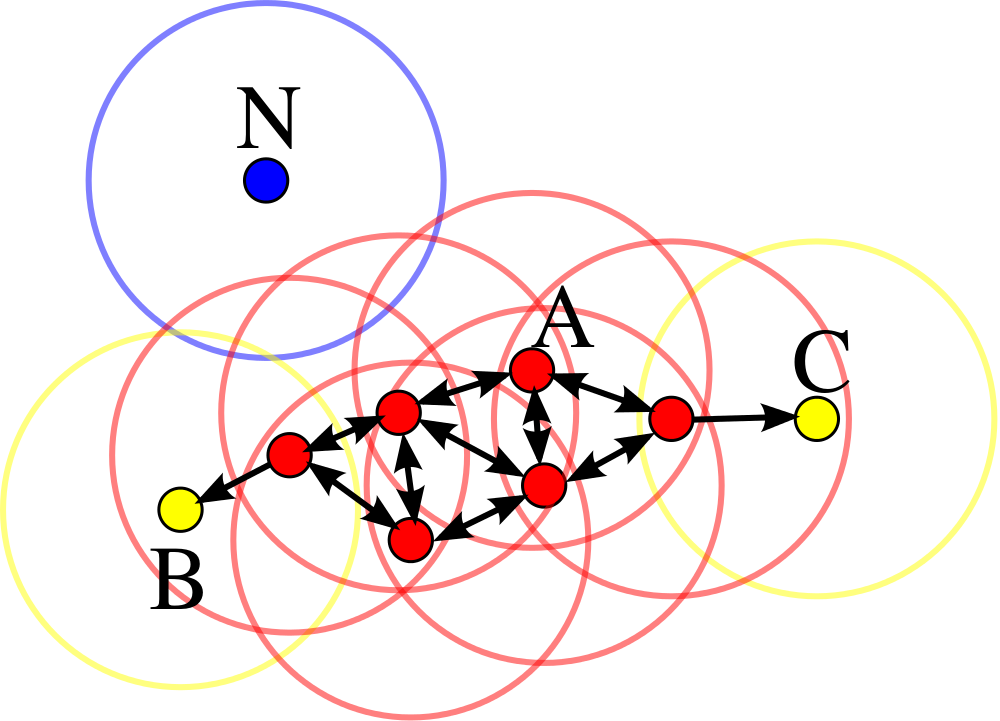
\includegraphics[width=0.8\linewidth]{DBSCAN-Illustration}
\caption{How \texttt{DBSCAN} selects the points in a cluster.}
\label{fig:DBSCAN}
\end{figure}

In this diagram [wikipedia], $minPts = 3$. Point A and the other red points are core points, because at least three points surround it in an $\epsilon$  radius. Because they are all reachable from one another, they form a single cluster. Points B and C are not core points, but are reachable from A (via other core points) and thus belong to the cluster as well. Point N is a noise point that is neither a core point nor density-reachable.

% when talking about code
\par It's worth noting a few optimizations that can be made to our implementation of this algorithm.
The distances between points, instead of being computed for each point ($O(N^2)$ lookups), can be computed in a type of tree structure ($O(N \log(N))$ lookups). Such position-tree structures are often called R-trees or R*-trees.
In addition, the \texttt{expandCluster} routine is only called from a single location, so it may be safely inlined.

%prediction under varying parameters

\subsection{FIDEPE}

\texttt{FIDEPE} (FInd DEnsity PEaks) algorithm \cite{FIDEPE} considers two criteria per point: Local Density and Minimum Distance to a point of higher density.

Local density ($\boldsymbol{\rho}$), is defined as the number of points $j$ in the "neighborbood"; points closer than $d_c$ from point $i$.
\begin{align*}
	\rho_i = \sum_j \chi(d_{ij}-d_c)
\end{align*}
where 
\begin{align*}
\chi(x)=
\begin{cases}
1 & x < 0 \\
0 & otherwise
\end{cases}
\end{align*}

Minimum Distance to a point of higher density (\textbf{Delta}) is self explanatory. 

\begin{align*}
	\delta_i = \text{min}_{j:\rho_j > \rho_i} (d_{ij})
\end{align*}

For the point of highest density though, \textbf{Delta} is just the maximum distance to another point.

\begin{align*}
	\delta_i = \text{max}_{j} (d_{ij})
\end{align*}

\begin{figure}[ht]
\centering
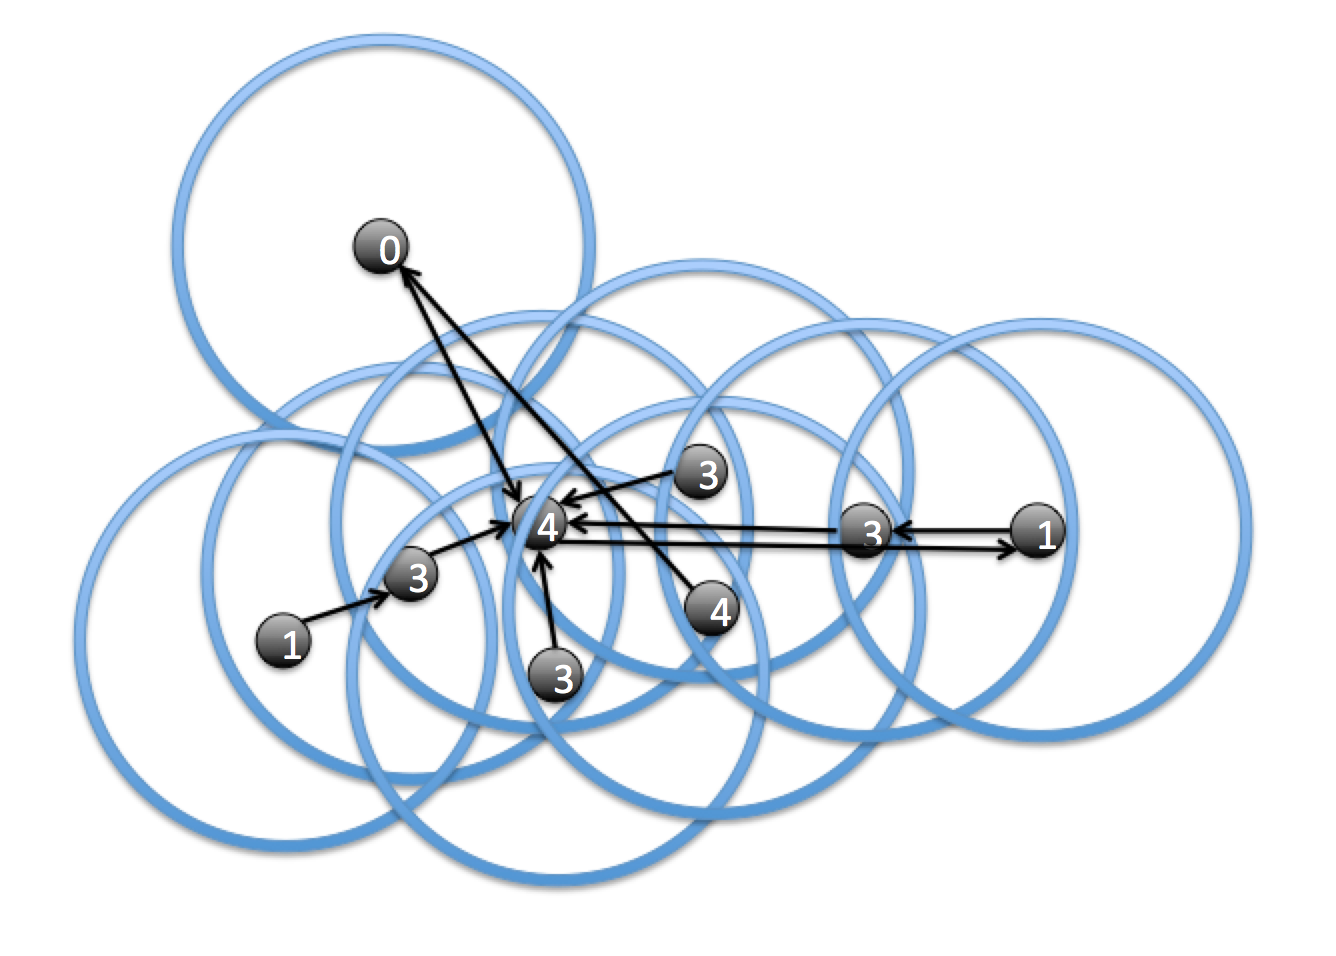
\includegraphics[width=0.8\linewidth]{fidepe_plots/FIDEPE}
\caption{How the \texttt{FIDEPE} algorithm identifies points in a cluster.}
\label{fig:FIDEPE}
\end{figure}


Figure \ref{fig:FIDEPE} shows a simple example of the quantities above described. Here \textbf{Rho} is marked as numbers above each of the points, the circles around them define a neighborhood of radius $d_c$ and the directed arrows are \textbf{Delta}.


Once this two quantities are defined for each point the algorithm identifies the points with both the highest \textbf{$\rho$} and \textbf{$\delta$} and tags them as cluster centers. The choice for how many of them fall under this criterion is not specified in the original code. We decided to select points 5 $\sigma$ away from the mean for \textbf{$\delta$} and 1 $\sigma$ away for \textbf{$\rho$}. This proved far away from robust.

\section{Plots}

\begin{figure}[ht]
\centering
%\includegraphics[scale=0.8]{plots/D31}
\caption{Our reference distributions.}
\label{fig:reference}
\end{figure}

\begin{figure}[ht]
\centering
\raisebox{0.75in}{\rotatebox[]{90}{Aggregation}}
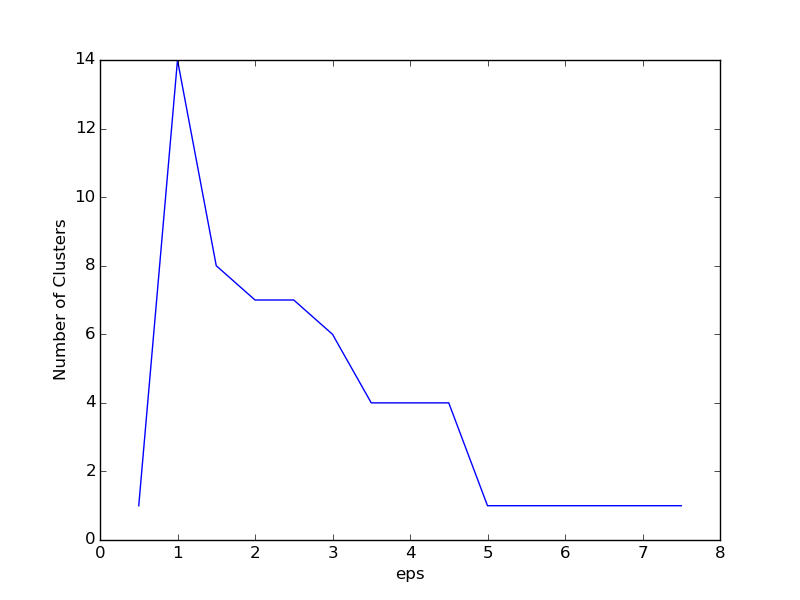
\includegraphics[width=0.35\linewidth]{plots/Aggregation_eps} 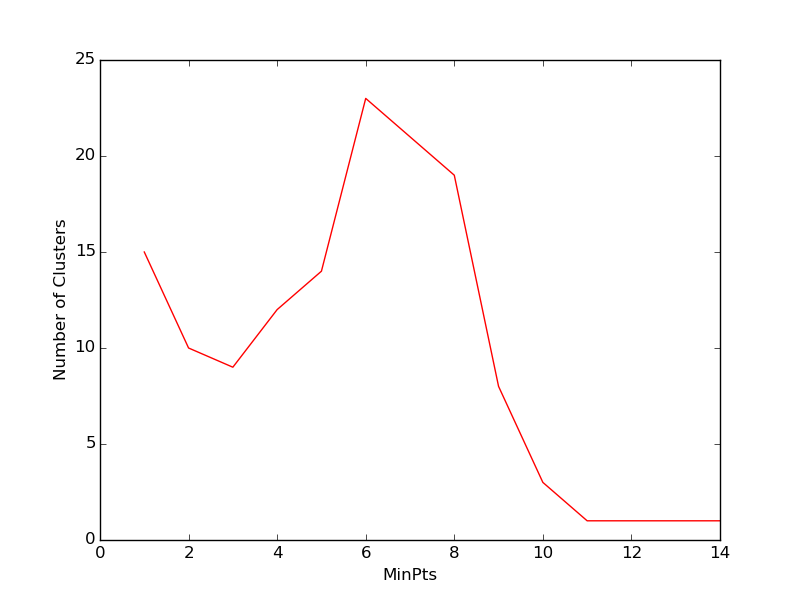
\includegraphics[width=0.35\linewidth]{plots/Aggregation_minpts} \\
\raisebox{0.75in}{\rotatebox[]{90}{Compound}}
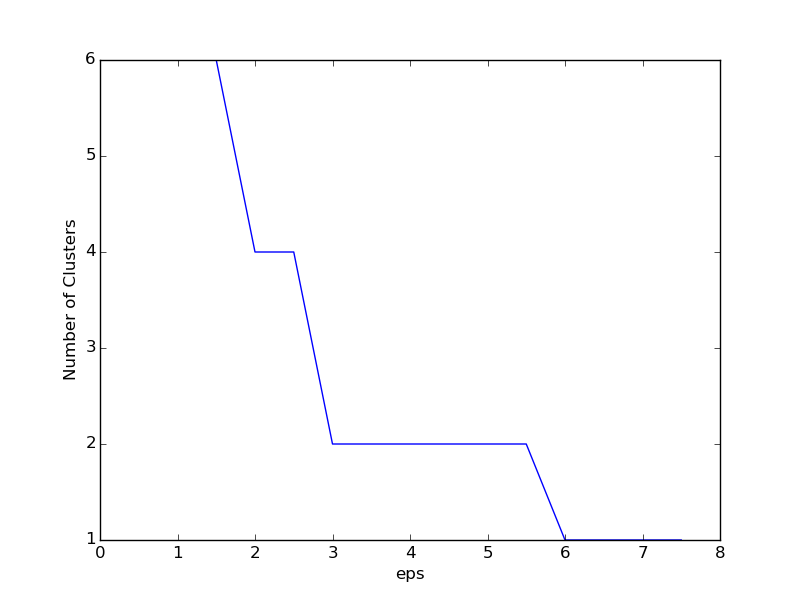
\includegraphics[width=0.35\linewidth]{plots/Compound_eps} 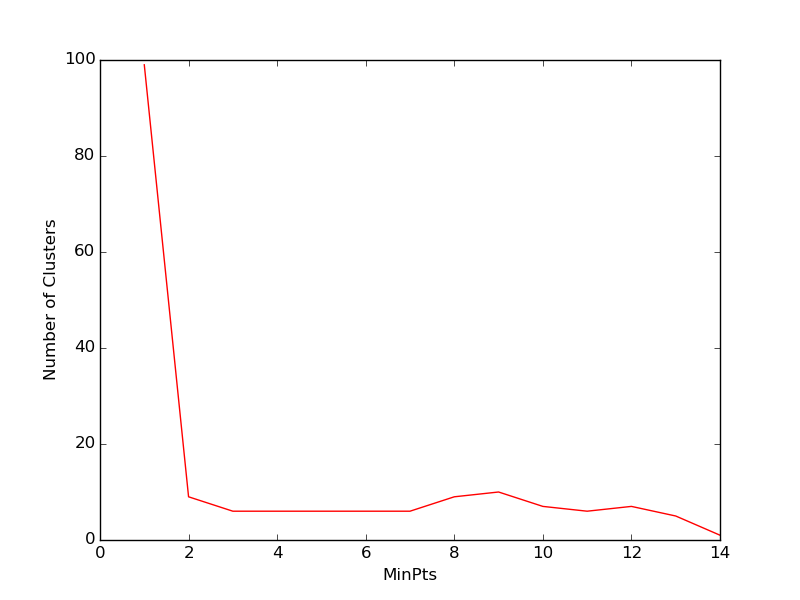
\includegraphics[width=0.35\linewidth]{plots/Compound_minpts} \\
\raisebox{0.75in}{\rotatebox[]{90}{D31}}
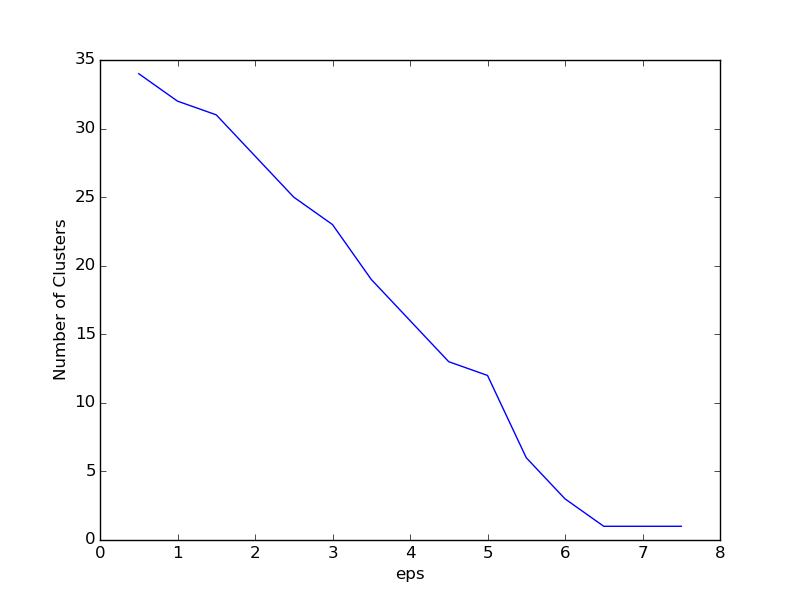
\includegraphics[width=0.35\linewidth]{plots/D31_eps}
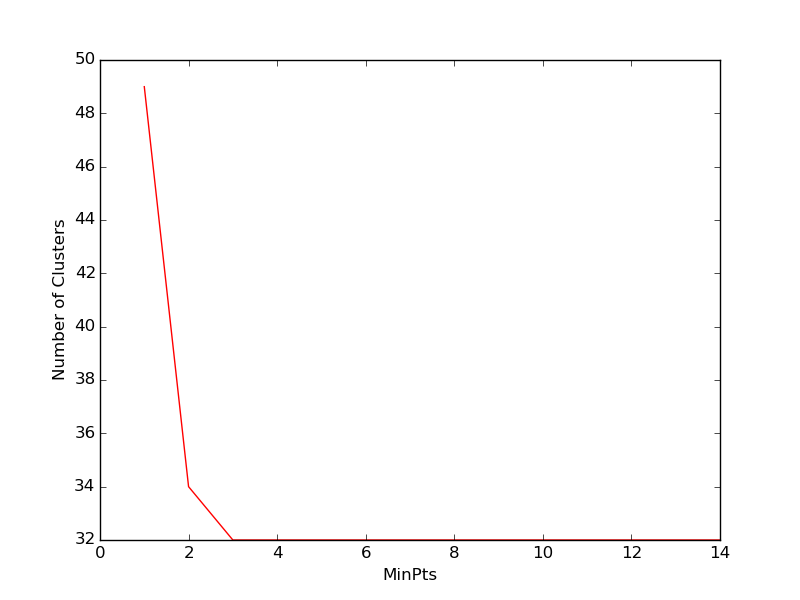
\includegraphics[width=0.35\linewidth]{plots/D31_minpts} \\
\raisebox{0.75in}{\rotatebox[]{90}{jain}}
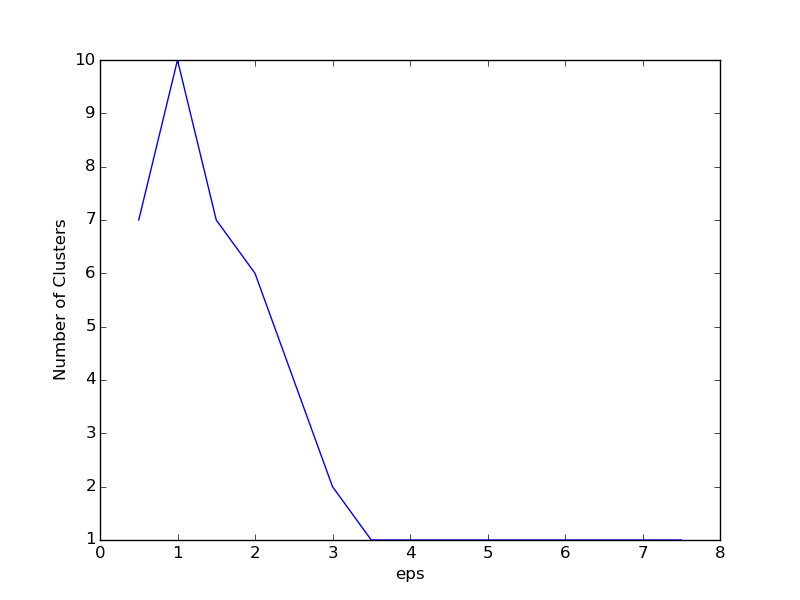
\includegraphics[width=0.35\linewidth]{plots/jain_eps}
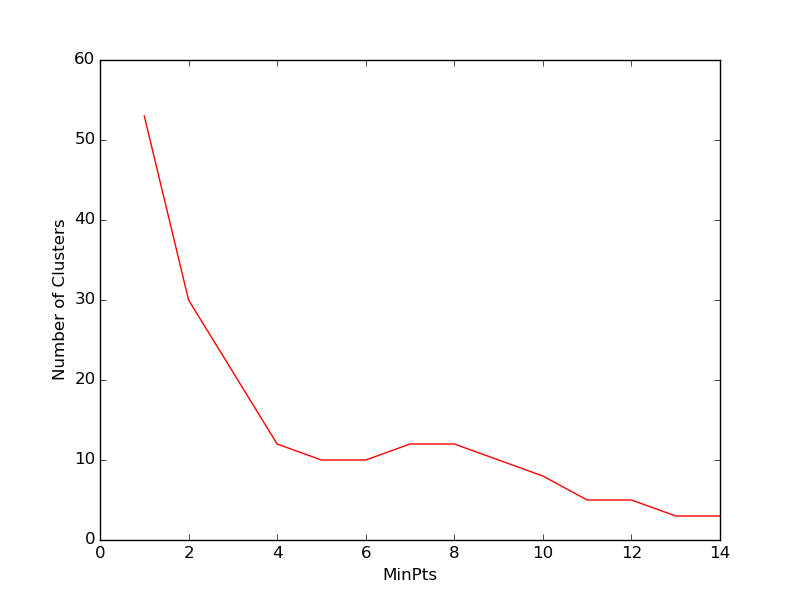
\includegraphics[width=0.35\linewidth]{plots/jain_minpts} \\
\raisebox{0.75in}{\rotatebox[]{90}{spiral}}
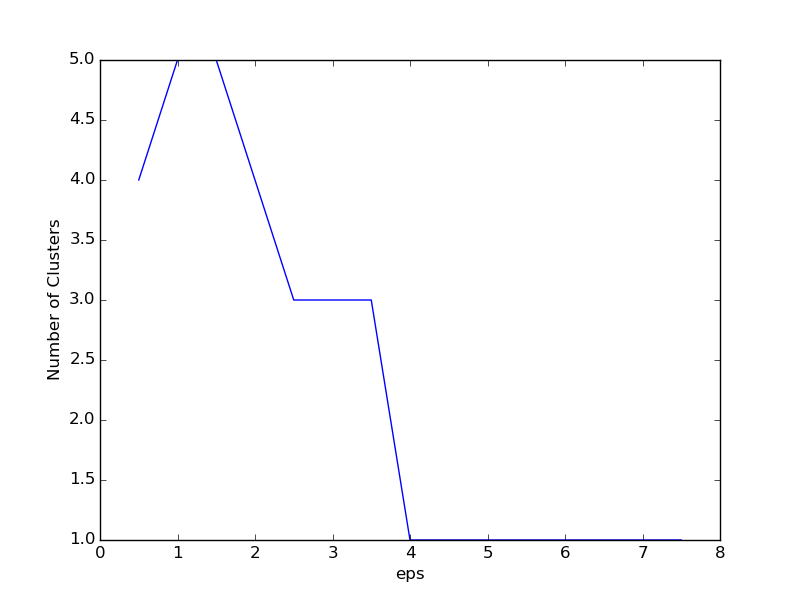
\includegraphics[width=0.35\linewidth]{plots/spiral_eps}
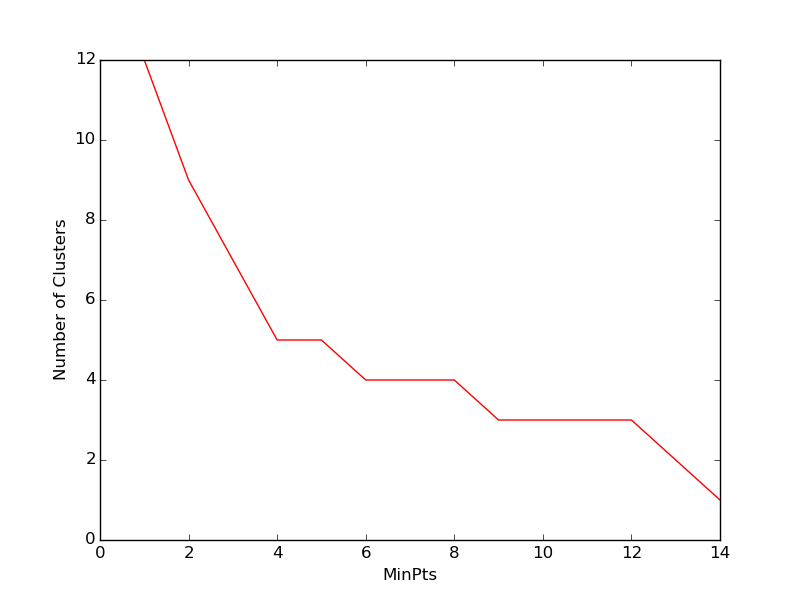
\includegraphics[width=0.35\linewidth]{plots/spiral_minpts}
\caption{(Left) The effects of varying the \texttt{eps} parameter of \texttt{DBSCAN} for all reference distributions. \\ 
(Right) The effects of varying the \texttt{MinPts} parameter of \texttt{DBSCAN}}.
\label{fig:DBSCANplots}
\end{figure}


\begin{figure}[ht]
\centering

\caption{The effects of varying the \texttt{FIDEPE} parameters.}
\label{fig:FIDPEPEplots}
\end{figure}


\section{Results}
\par Referencing Figure \ref{fig:DBSCANplots}, the \texttt{DBSCAN} algorithm does not seem particularly robust to variation in either \texttt{eps} or \texttt{MinPts}. Our proposed mechanism for objectively identifying the number of active clusters appears to fail in almost all test cases. The \texttt{spiral} dataset seems to be the exception, in that the flattest regions of the plots occur at the true number of clusters. The most densely clustered dataset, \texttt{D31}, converges in the range of \texttt{MinPts} plotted to the true cluster number, but fails to plateau in the range of \texttt{eps} plotted. (Describe other datasets?)
\par Referencing Figure \ref{fig:FIDPEPEplots}, the \texttt{FIDEPE} algorithm is extremely sensitive to the user's choice of parameters. This may be to our ad hoc choice of the standard deviation clustering parameter. More.

\par Our choice not to explore the full parameter space for these plots likely has contributed to our inability to find the peak cluster plateau we na\"\i vely expect. However, there is no guarantee of any sort of robustness in these algorithms. It may possible to construct datasets with a plateau on a false cluster number somewhere in the parameter space. We leave these questions for future work, now only concluding that our heuristic is useful in some nonzero percentage of typical datasets.
\clearpage
\bibliographystyle{plain}
\bibliography{research}

\end{document}
